\documentclass[11pt]{article}

% ============================================================
% CIS 3296 — Software Design
% Individual Project Proposal
% Temple University Japan
%
% This project works in Overleaf or in a local LaTeX installation.
% ============================================================

% ---------- Page layout and typography ----------
\usepackage[a4paper,margin=25mm]{geometry}
\usepackage[T1]{fontenc}
\usepackage{lmodern}
\usepackage{microtype}
\usepackage{parskip}
\usepackage{setspace}

% ---------- Figures and tables ----------
\usepackage{graphicx}
\usepackage{float}
\usepackage{booktabs}
\usepackage{tabularx}
\usepackage{array}
\usepackage{caption}

% ---------- Lists, color, links ----------
\usepackage{enumitem}
\usepackage{xcolor}
\usepackage{xurl}
\usepackage{hyperref}
\usepackage[nameinlink,noabbrev]{cleveref}

% ---------- Bibliography ----------
\usepackage{csquotes}
\usepackage[
    backend=biber,
    style=ieee,
    sorting=none
]{biblatex}
\addbibresource{references.bib}

% ---------- Page style ----------
\usepackage{fancyhdr}
\usepackage{titlesec}

\definecolor{templeburgundy}{HTML}{9D2235}
\definecolor{darkgray}{HTML}{3F3F3F}
\definecolor{midgray}{HTML}{6D6D6D}

\setstretch{1.05}
\setlist[itemize]{leftmargin=1.5em}
\setlist[enumerate]{leftmargin=1.6em}

\captionsetup{
    font=small,
    labelfont=bf
}

\hypersetup{
    colorlinks=true,
    linkcolor=templeburgundy,
    citecolor=templeburgundy,
    urlcolor=templeburgundy,
    pdftitle={CIS 3296 Individual Project Proposal}
}

\titleformat{\section}
  {\large\bfseries\color{templeburgundy}}
  {\thesection.}{0.55em}{}

\titleformat{\subsection}
  {\normalsize\bfseries\color{darkgray}}
  {\thesubsection.}{0.55em}{}

\pagestyle{fancy}
\fancyhf{}
\lhead{\small CIS 3296 — Software Design}
\rhead{\small Individual Project Proposal}
\cfoot{\small \thepage}
\renewcommand{\headrulewidth}{0.4pt}

% ============================================================
% Student information — edit these four lines
% ============================================================
\newcommand{\projecttitle}{MakeMe}
\newcommand{\studentname}{Karl Fernandez}
\newcommand{\proposaltype}{Group Report}
% \newcommand{\submissiondate}{October 2026}

% Figure placeholder used until an image file is added.
\newcommand{\figureplaceholder}[2]{%
    \fbox{%
        \parbox[c][#1][c]{0.88\linewidth}{%
            \centering\color{midgray}\small #2
        }%
    }%
}

\begin{document}

% ============================================================
% Title page
% ============================================================
\begin{titlepage}
    \thispagestyle{empty}
    \centering

    \IfFileExists{figures/temple-logo.png}{
        
\includegraphics[width=0.46\textwidth]{figures/temple-logo.png}
    }{
        {\Large\bfseries Temple University Japan\par}
    }

    \vspace{0.45cm}
    {\color{templeburgundy}\rule{0.76\textwidth}{1.1pt}}

    \vfill

    {\Large\bfseries \proposaltype\par}

    \vspace{1.0cm}

    {\huge\bfseries \projecttitle \par}

    \vspace{1.5cm}

    \begin{tabular}{>{\bfseries}r l}
        Team: 
            & Karl Fernandez \\
            & Moe Odaki \\ 
            & Scout Peterson \\[3pt]
        Github: & \url{https://github.com/kidevil1290/makeme} \\
        Date: & November 26, 2026 \\
    \end{tabular}

    \vfill

    {\small CIS 3296 — Software Design\par}
\end{titlepage}

% ============================================================
% 1. Project Summary and Motivation
% ============================================================
\section{Abstract}
\textit{Maintaining consistent exercise habits over an extended period can be challenging,
particularly when fitness progress is primarily represented through numerical data.
MakeMe is a gamified fitness-tracking application designed to address this challenge by
integrating personalized avatar progression into the fitness-tracking experience.
The application translates users' real-world activities into visual changes in a personalized
virtual character, with its initial minimum viable product (MVP) incorporating four core
components: character customization, workout logging, muscle-specific progression,
and a 90-day game cycle. Character customization allows users' to personalize their avatars,
establishing a stronger sense of connection with their virtual representations,
while the 90-day cycle introduces a structured progression period that provides a longer-term
objective. At the core of this system, workout logging records users' training activity,
which drives muscle-specific growth in their avatars. This creates a direct relationship
between real-world exercise and avatar development, allowing users' to visualize
how their individual training activities contribute to their avatars progression.
Through these interconnected mechanics, MakeMe aims to provide users' with a more engaging
representation of their fitness progress and encourage consistent exercise through
game-inspired progression mechanics.}

\section{Introduction}

\subsection{Background and Context}
Conventional fitness-tracking applications provide users with a range of tools to monitor
and manage their physical activities. Activities that were traditionally recorded through
handwritten logs and manual calculations can now be conveniently organized within digital
platforms, allowing users to track workout frequency, monitor performance, and review their 
progress over time. These features provide valuable feedback and help users establish a
structured approach to their fitness routines. Across many of these applications,
numerical statistics remain a central method of presenting users' progress. However,
while these measurements provide useful information, they offer limited opportunities
for users to visually identify with their progress or develop an aspirational connection
with their fitness goals. As a result, the ability to monitor fitness activity does not
necessarily translate into sustained motivation or consistent exercise habits. 

One potential approach to making fitness progress more engaging is through the use of
personalized avatars. These avatars can serve as visual representations of users,
gradually developing alongside their real-world physical activities. By allowing users
to customize their avatars, applications can create opportunities for stronger
self-identification, making the avatar's development more personally meaningful.
Furthermore, allowing these characters to develop toward an idealized physique introduces
an aspirational element, giving users a visual representation of what they may hope to
achieve through their own fitness journey. Through this combination of self-representation
and aspiration, avatars can provide users with a more personal and engaging
connection to their fitness goals.

Building upon these concepts, MakeMe is a gamified fitness-tracking application designed
to connect users' real-world exercise activities with the development of a personalized
avatar. The initial minimum viable product (MVP) focuses on four core components:
character customization, workout logging, muscle-specific progression, and a 90-day game
cycle. Users can personalize their avatars and record their workout activities,
which contribute to the gradual development of specific muscle groups within the avatar.
Rather than representing physical development as a generalized progression, MakeMe aims
to reflect users' individual training habits through muscle-specific visual changes. This
progression is further structured around a 90-day cycle, providing users with a defined
period in which to develop their avatars and work toward their fitness goals. By combining
workout tracking, character customization, and visual progression, MakeMe seeks to create
a more personalized and game-inspired approach to monitoring fitness development.

\subsection{Motivation and Problem Statement}
Despite the availability of fitness-tracking applications, maintaining consistent
engagement with exercise routines remains a challenge for many individuals. Recording
workouts and monitoring physical activity can help users organize their fitness routines,
but these activities alone do not necessarily provide a compelling reason to remain engaged
over an extended period. There is an opportunity to explore how game-inspired progression
systems can make continued participation more meaningful by connecting users' exercise
efforts with a sense of personal development. The challenge addressed by MakeMe is to design
an application that translates individual workout activities into personalized,
muscle-specific avatar progression while providing a structured experience through its
90-day game cycle.

The motivation behind developing MakeMe stems from the opportunity to make fitness
tracking more engaging through concepts commonly found in video games.
By incorporating personalized character development into the fitness-tracking
experience, the project explores how users can establish a stronger connection
with their fitness goals through virtual self-representation and aspirational
progression. Rather than focusing exclusively on recording physical activities,
MakeMe aims to provide users with a visual representation of their training efforts,
where individual workouts contribute to the gradual development of a character
they have personalized. This approach seeks to make fitness progression more
personally meaningful while introducing game-inspired mechanics that may
encourage users to remain engaged with their exercise routines. Ultimately,
the project aims to explore how principles of character customization and progression
can be applied to fitness applications to support a more engaging approach to exercise tracking.
\subsection{Project Goals and Objectives}
MakeMe's primary goal is to explore how conventional fitness-tracking functionality
can be extended through game-inspired character progression. By incorporating personalized
virtual representations into the fitness-tracking experience, the project aims to establish
a more engaging approach to visualizing users' fitness development. The initial MVP serves
as the foundation for this broader vision, establishing the essential functionality and
progression systems upon which additional features can be developed and integrated in the future.

To establish this foundation, the project pursues the following objectives.
\begin{enumerate}
    \item Develop a Personalized Avatar System: Implement a customizable virtual
    character whose appearance can be personalized by users with individual muscle groups
    that develops independently through recorded workout activities.
    
    \item Integrate Core Fitness-Tracking Functionality: Implement essential
    workout-logging functionality that allows users to record their exercise
    activities serving as the foundation for the application's avatar progression system.

    \item Establish a Structured Progression System: Develop a 90-day progression
    cycle that provides users with a defined period to track their activities, observe
    avatar development, and work toward longer-term fitness goals.

\end{enumerate}

\section{Literature Review and Related Work}

\subsection{Relevant Resrearch and Existing Products}
MakeMe’s avatar system draws on virtual self-modeling through vicarious reinforcement by Fox
and Bailenson, which explored how observing virtual representation of oneself receiving reinforcement
would influence exercise behavior \cite{fox2009VRS}. However, their research used virtual representation that
resembled the participants, whereas MakeMe features fantasy-based character development that would
later skew away from the users physical appearance. This distinction is intentional, as MakeMe allows
users to watch their avatars develop into increasingly muscular and powerful characters, potentially
inspiring them to aspire to the strength and appearance of their virtual counterparts, motivating them
to maintain healthy habits. This design aligns the concept of wishful identification mentioned in the
review research by Praetorius and Gorlich on the Proteus Effect, which describes how an avatar's characteristics
may influence a users behavior and self-perception \cite{praetorius2020avatars}.Drawing on these concepts, MakeMe’s
avatar system is designed around two complementary forms of progression: reflective and aspirational. Where the development
of the avatar is a direct reflection of users actions, while aspirational progression allows the avatar to evolve towards
an idolized physique that users may wish to achieve themselves. While existing research does not directly establish
a link between avatar progression and the development of healthy habits, incorporating them may still offer
motivational benefits compared with health tracking applications without an avatar.

Although ranking of the top 10 fitness trackers may vary due to subjective
reviews and potential biases, many of them can be broadly classified into three categories based on their approaches
to fitness tracking and gamification.

Category 1 consists of conventional fitness trackers that incorporate little to no gamification,
focusing primarily on workouts, activity logging, and social features \cite{hall2026bestfitnessapps, herman2026bestfitnessapps}. Their
popularity suggests that stand-alone fitness monitoring remains an established approach to helping users
track their progress and maintain their fitness routine. However, this category represents only one approach
to fitness tracking and does not establish whether users would benefit from engaging or game-oriented alternatives.

Category 2 consists of challenge-based gamified fitness trackers that are oriented to encourage physical
activity through step-count goals, competitions, social challenges, and real-world incentives. In 2020, (Neupane et al.)
reviewed 103 gamified fitness tracker apps and found that challenges, competition and social influence frequently
appeared together, while social features played a central role across nearly every identified game genre \cite{neupane2020review}.
These findings demonstrate how conventional activity tracking can be enhanced with game mechanics that encourage
users to remain active through external rewards, social interaction, and competition. However, this approach primarily
builds on existing fitness tracking activities rather than making exercise part of a broader, evolving game experience.

Category 3 consists of stand-alone games that integrate physical activity directly into gameplay, encouraging
users to exercise as they pursue in-game objectives. Games such as PokemonGO and Wii Sports demonstrate the popularity
of this approach making physical activity more engaging through exploration and interactive gameplay \cite{koh2026motivational, yim2007using}.
In these games, physical avtivity is not simply a means of tracking progress but an integral part of the game itself. Players are motivated to move, explore, and engage with their environment to achieve in-game goals.
However, research on PokemonGO suggests that increased in physical activity may be short-lived, highlighting the challenge
of sustaining user engagement and long-term exercise habits.

\subsection{Comparison With the Proposed Project}
Initially, MakeMe was envisioned as an application that would combine elements from the three
approaches discussed above, bringing together conventional fitness tracking, gamification,
and interactive gameplay. However, as the project developed, its scope was refined to focus
on a more specific aspect of the fitness-tracking experience: connecting users' workout
activities with the development of their avatars. Rather than attempting to incorporate
the various challenges, social features, and gameplay mechanics found in existing solutions,
the current MVP places its emphasis on workout logging and muscle-specific avatar progression.
Through this approach, recorded exercise activities directly contribute to the development of
corresponding muscle groups within a personalized character. This shift allows MakeMe to
concentrate on its central design concept providing users with a visual representation of
their training efforts through an avatar that develops alongside their fitness journey.
\section{Project Requirements}
\subsection{Product Vision and Scope}
MakeMe is a gamified fitness-tracking application that aims to connect users’ real-world fitness
activities to a developing personalized avatar. The application is designed around the idea that
progress from workouts can be represented through a character that gradually develops alongside
the user’s training habits. Rather than relying exclusively on numerical workout records, MakeMe
complements them with visual character development to provide users with another way to observe
their fitness progress.

The MVP focuses on four main components: character customization, workout logging, muscle-specific
avatar progression, and a 90-day progression cycle. Users can personalize their avatar upon
creation before recording their workouts. Based on the recorded workouts, the avatars
corresponding muscle groups gradually develops, allowing different areas of the character
to progress according to the user’s training habits. The 90-day cycle provides a structured
period for users to work toward their fitness goals, with the opportunity to ascend into a
new cycle, receiving badges to recognize their accomplishments.

The original conceived idea was a broader system that considered nutrition, hydration, and sleep
tracking, alongside additional mechanics such as avatar decay, recovery, and bulk progression.
However, these features have been excluded from the initial MVP due to the interest of time and
the amount of resources they required. Several of the proposed systems also depended on extensive
visual assets and additional implementation, which would significantly increase the project’s
development complexity. Ultimately, MakeMe concluded to prioritize the core workout and avatar
progression mechanics before considering integrating additional features. This narrower scope
allowed the project to concentrate on its primary mechanic while establishing a foundation for
future expansion.

\subsection{High-Level Requirements}
\begin{itemize}
    \item \textbf{R1.} Initial Avatar Set Up. The system will allow users to personalize their avatars head
        at creation and a short survey will be used to establish the avatars initial baseline.
    \item \textbf{R2.} Workout Logging. A dedicated workout logger will collect
        duration, select muscle group, and intensity level from user input.
    \item \textbf{R3.} Muscle-Specific Growth. The system will take the logged data from workout logger
        and calculate and apply growth to the corresponding muscles.
    \item \textbf{R4.} Avatar Display. The system will display the avatar's current appearance and muscle development
    \item \textbf{R5.} 90-day Cycle. The system will track user progression within 90-day cycle.
    \item \textbf{R6.} Ascension System. The system will allow users to ascend into a new progression cycle
        upon completion of the current cycle.
    \item \textbf{R7.} Reward System. The system will reward users with a badge after ascension.
\end{itemize}
\subsection{Target Users and 2 to 5 personas}

\section{System Design}

\subsection{System Architecture}
\subsection{Use Case Diagram}
\subsection{UML Class Diagram}
\subsection{Sequence Diagram}
\subsection{Design Patterns and Justification for Their Use}

\section{Implementation and Proof of Concept}

\subsection{Tools and Technologies}
\subsection{Implementation of the Main Features}
\section{Required Resources and Feasibility}

\subsection{Hardware, Software, and Other Resources}
\subsection{Feasibility Within the Avaialble Time and Resources}

\section{Results and Discussion}

\subsection{Proposed Features and Their Completion Status}
\subsection{Testing and Results}
\subsection{Challenges, Limitations, and Reasons for Incomplete Features}

\section{Conclusion and Future Work}
\subsection{Summary of Achievements}
\subsection{Possible Improvements and Extensions}

\section{References}

\section{Implementation Goals and Scope}

\subsection{Implementation Goals}

% State 3–5 concrete goals.
% Goals should describe observable capabilities rather than vague intentions.


\subsection{Core Functional Requirements}

% List 4–6 core functional requirements.
% Focus on externally visible behavior rather than implementation details.

\begin{itemize}
    \item \textbf{R1.} Initial Avatar Set Up. The system will collect initial user data through a survey and use the response as the avatars baseline.
    \item \textbf{R2.} Workout Logging and Muscle-Specific Growth. A dedicated workout logger that collects duration, selected exercised
         body parts, and intensity level from user input. The system uses this input to calculate growth for selected body parts.
    \item \textbf{R3.} Workout Streak Tracking: The system maintains a workout streak using a 48-interval after a workout log,
         allowing users to include rest days without automatically breaking their streaks.
    \item \textbf{R4.} Avatar Decay. The avatar decays continuously and can be accelerated through poor meal logging habits.
         This system balances growth from workout logging to simulate a semi-realistic growth rate. 
    \item \textbf{R5.} Avatar State System: The system updates the avatars’ appearance and state based on the user’s logged habits.
    \item \textbf{R6.} Habit Logging. Allows users to record meals, hydration and sleep that contributes to avatars state system and progression.
    \item \textbf{R7.} Bulk Progression. Accumulated throughout the cycle and reads through macro report from macro tracker and calculates
         progression in clean bulk and dirty bulk that influence the avatars overall appearance.
    \item \textbf{R8.} Recovery and Revival. Prolonged period of inactivity can result to the avatars death. A recovery system
         detects the users return within three stages that determines recovery state from initial return work out logging to a three-day
          workout streak. The avatar loses all its progress and will return to its initial state.
    \item \textbf{R9.} Cycle Completion and Summary. The system tracks a 90-day cycle to simulate a three-month transformation and presents
         a summary of the user’s activity, avatar development, and achievements.
    \item \textbf{R10.} Ascension System. Determines if the user has completed their long-term goals and allows the user to begin a new cycle,
        including a new initial survey and avatar baseline. A badge or title will be rewarded with each ascension.
    \item \textbf{R11.} Limited rewards such as badges or cosmetic items for completing certain milestones.
\end{itemize}

\subsection{Initial Scope}

\textbf{In scope.}
The initial version of MakeMe will focus on implementing the avatar’s initial configuration, muscle-specific growth, workout logging,
     streak system, and time-based decay. It will also include habit logging, supporting avatars conditional states and bulk progression.
        A 90-day progression cycle, cycle-completion and summary that provides the user a long term objective.

\medskip

\textbf{Out of scope.}
The initial implementation will exclude extensive equipment collections, multiplayer features, competitive leaderboards,
     and advanced social systems. Character customization, avatar appearance states, and visual progression will also be
        limited to a predefined set of options. Additionally, the application will not provide medical diagnoses or claim
     that avatar development accurately represents a user's real body composition or physical health.

% ============================================================
% 4. Initial Design
% ============================================================
\section{Initial Design}

\subsection{Use-Case Diagram}

% Include the main actors and 4–6 meaningful user-level use cases.
% Actors remain outside the system boundary.
% Use cases should represent user goals, not Java methods or classes.
%
% Export the diagram as PDF when possible and save it as:
%   figures/use-case-diagram.pdf

The primary actor is the User, who interacts with the application to track health habits and monitor personal progress. The user's goals
include creating an initial avatar, logging health related-activities, viewing the avatars visual development as it changes in stature,
appearance, and condition in response to their habits, reviewing macronutrient summaries and cycle progress, avatar personalization,
and managing health goals. These use cases illustrate how MakeMe combines health habit tracking with visual character progression
to encourage users to maintain healthy routeines throughout the 90-day progression cycle represented in \cref{fig:usecase}.

\begin{figure}[H]
    \centering
    \IfFileExists{figures/use-case-diagram.pdf}{
        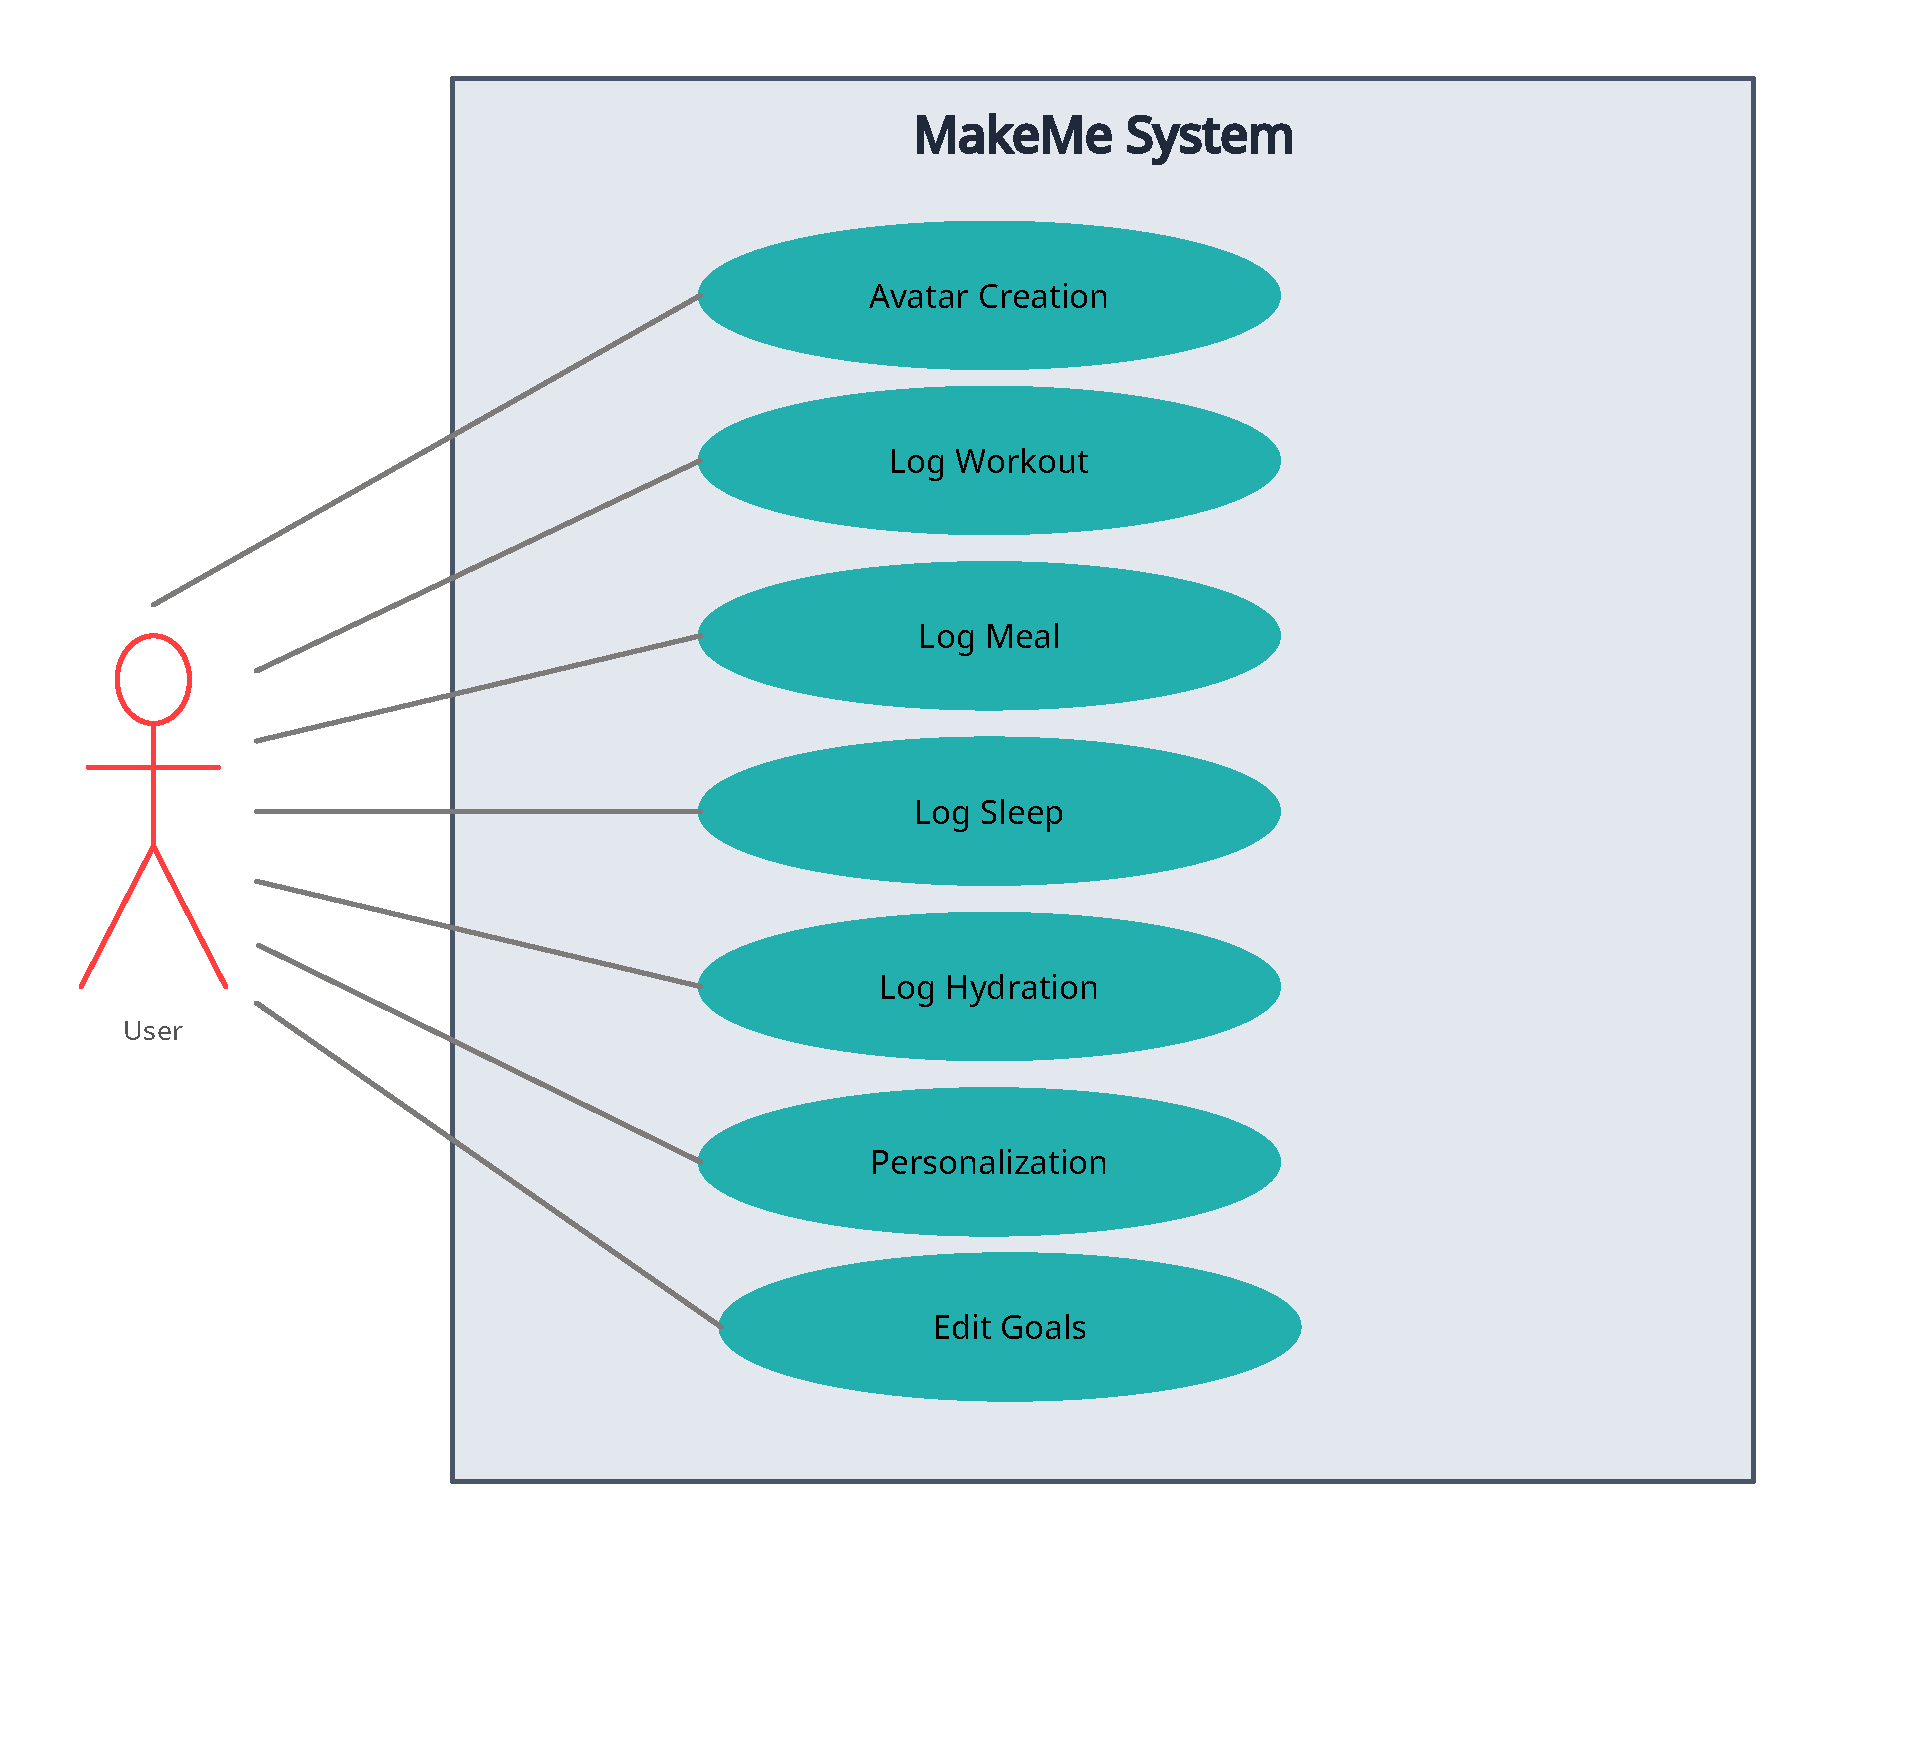
\includegraphics[width=0.92\linewidth]{figures/use-case-diagram.pdf}
    }{
        \figureplaceholder{55mm}{Add \texttt{figures/use-case-diagram.pdf}}
    }
    \caption{Initial use-case diagram for the proposed system.}
    \label{fig:usecase}
\end{figure}

\subsection{Class Diagram}

% Show:
%   - the main classes and/or interfaces
%   - important attributes and operations where appropriate
%   - meaningful relationships
%   - relevant multiplicities
%
% Do not invent inheritance only to make the diagram more complex.
%
% Export as:
%   figures/class-diagram.pdf

The class diagram shown in \cref{fig:classdiagram} organizes MakeMe into classes responsible for user profiles, avatar progression, workout logging,
     nutrition tracking, and health habits. The Avatar and BodyPart classes manage visual development, while BulkProgression
        and the streak classes track consistency and progress. The CycleManager manages the 90-day progression cycle,
        and the RewardSystem handles milestone rewards and equipment unlocks. Relationships between classes primarily
        use associations and composition, while inheritance connects the abstract Streak class to WorkoutStreak and MealStreak.
        Enumerations define predefined states and options used throughout the system.

\begin{figure}[H]
    \centering
    \IfFileExists{figures/class-diagram.pdf}{
        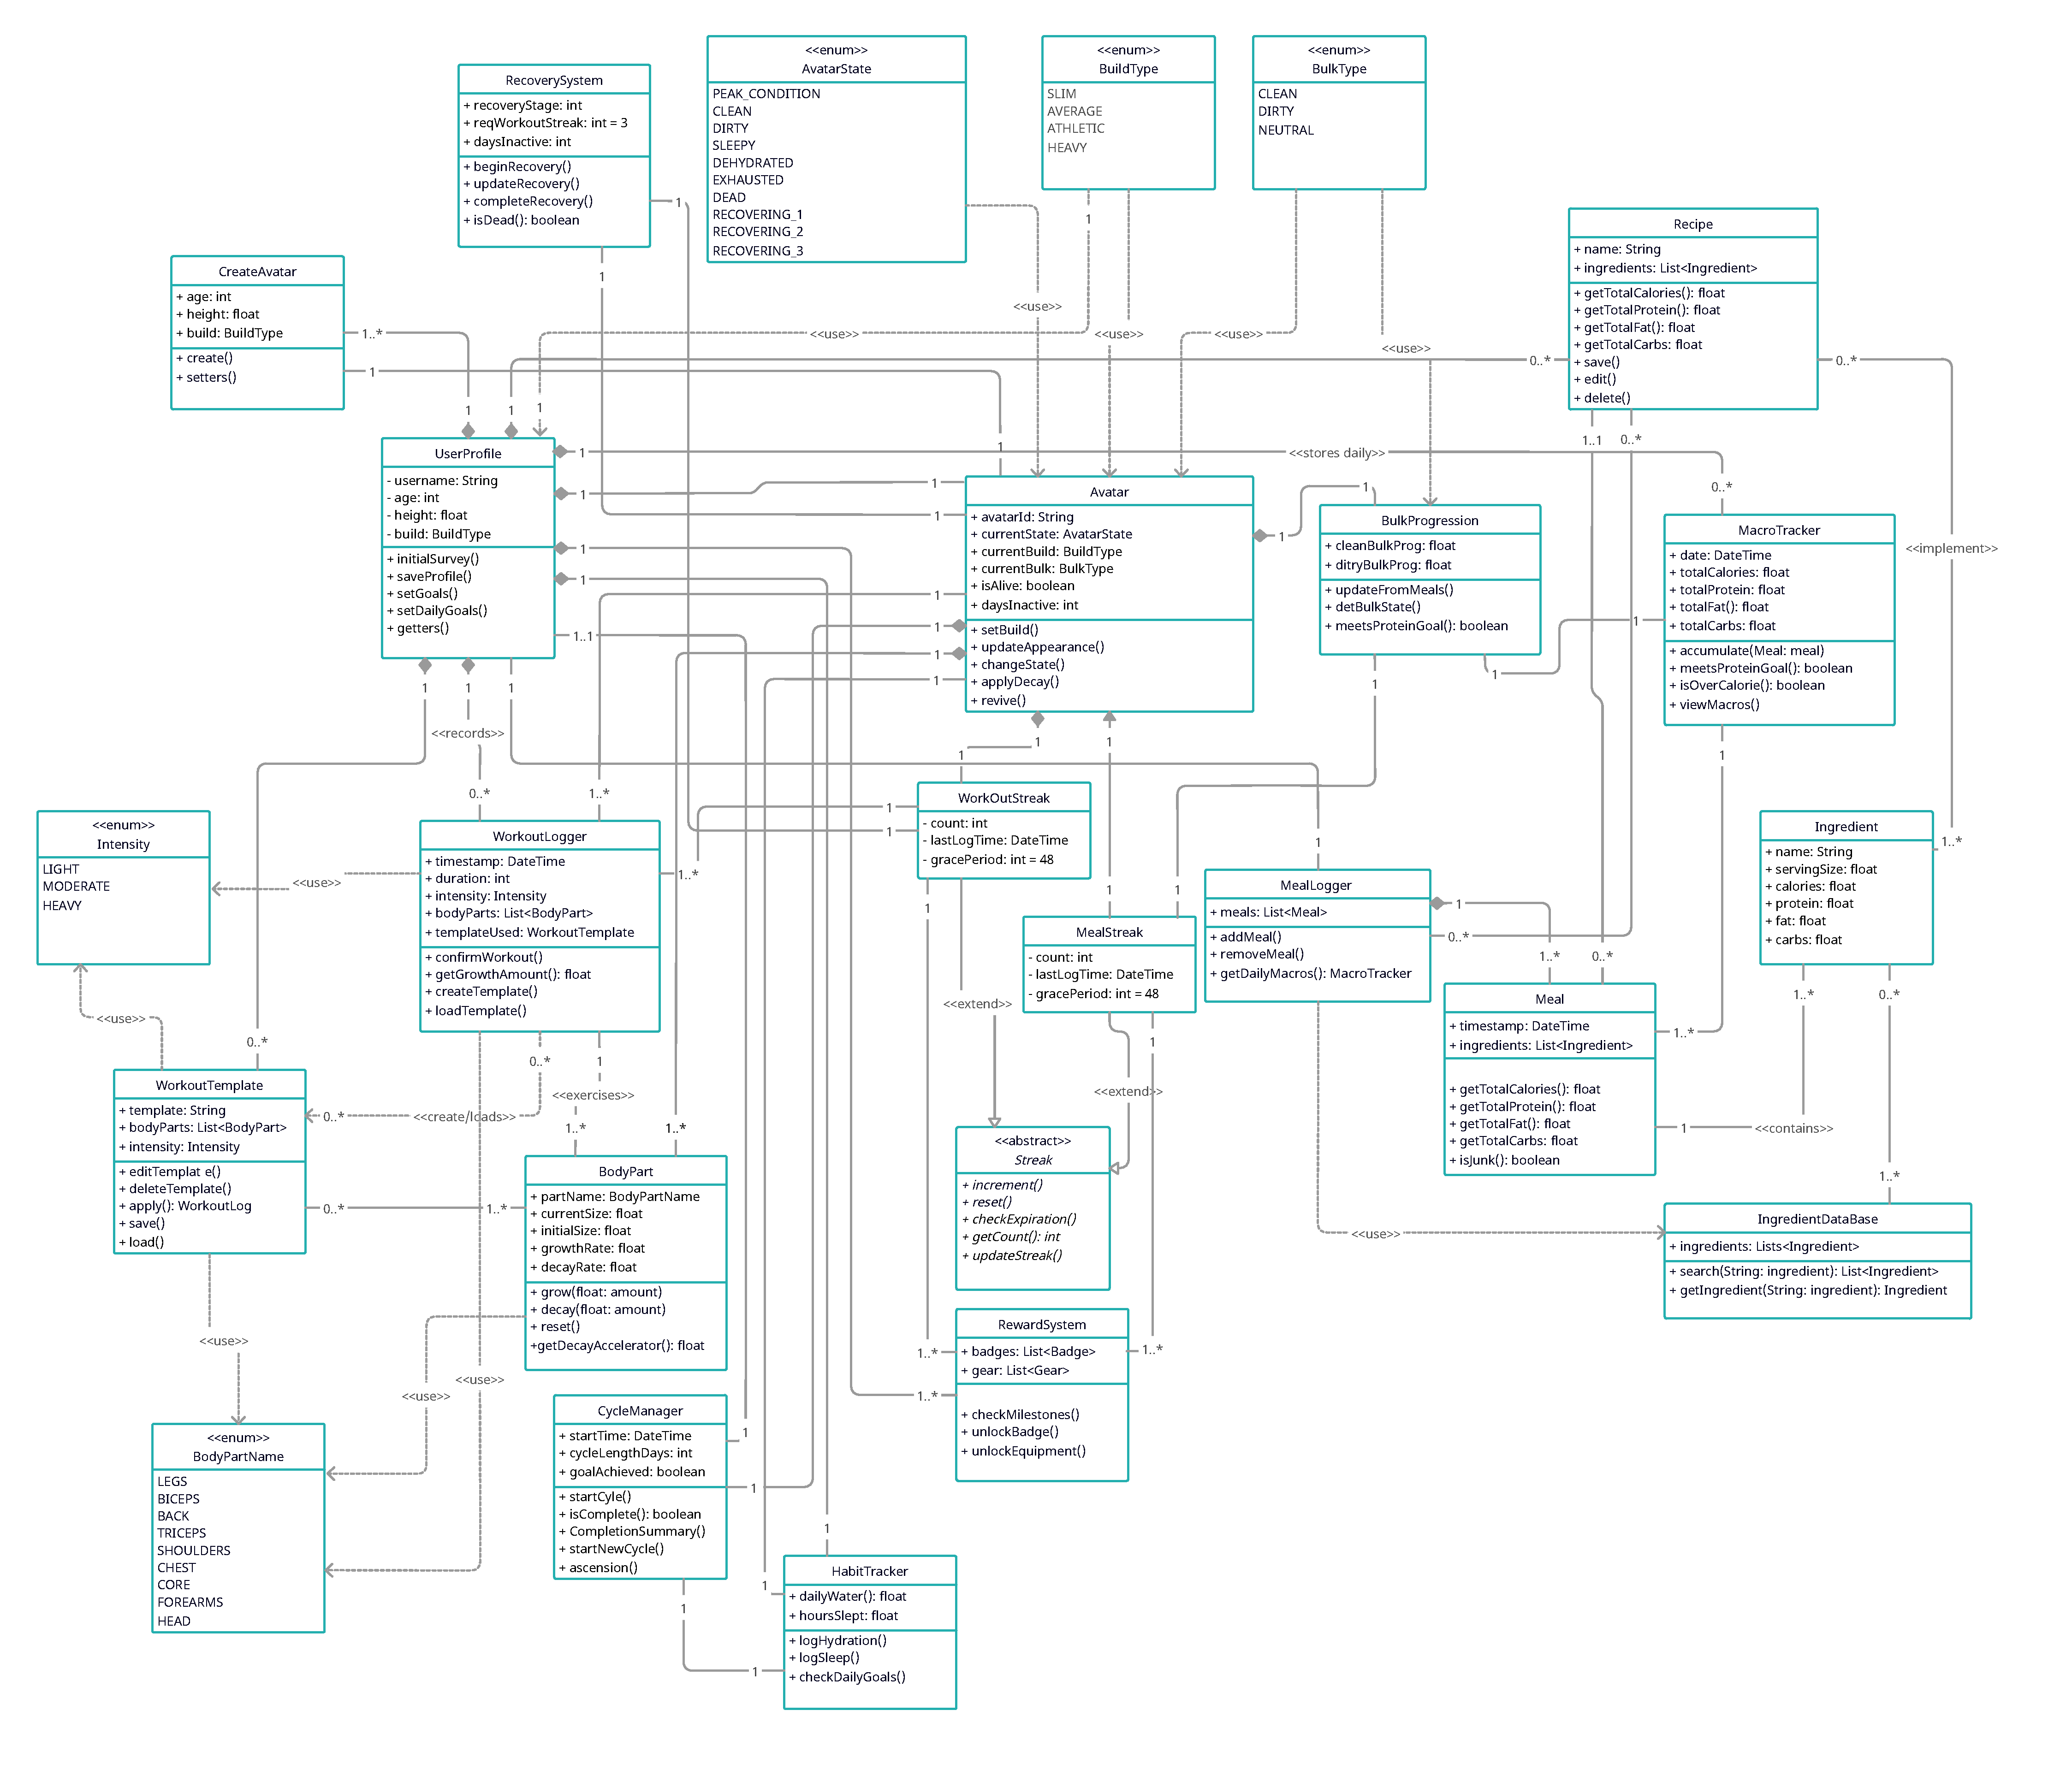
\includegraphics[width=0.92\linewidth]{figures/class-diagram.pdf}
    }{
        \figureplaceholder{55mm}{Add \texttt{figures/class-diagram.pdf}}
    }
    \caption{Initial UML class diagram for the proposed system.}
    \label{fig:classdiagram}
\end{figure}

% ============================================================
% 5. Feasibility and Supporting Evidence
% ============================================================
\section{Feasibility and Supporting Evidence}

% Describe the technologies relevant to the proposal:
% language, framework, libraries, APIs, database/data source,
% external services, operating environment, or hardware.
%
% Explain why the project is feasible within the course.
%
% Include at least one supporting figure beyond the UML diagrams, such as:
%   - UI mockup
%   - architecture sketch
%   - API result
%   - screenshot of an existing system/component
%   - small prototype or technical experiment
%
% Clearly distinguish a proposed design from a tested result

\textit{The technical feasibility of MakeMe depends primarily on developing its avatar progression system, which
    is expected to require the largest portion of development time. Unlike conventional fitness applications that
    display numerical statistics, MakeMe aims to visually represent progress through body-part-specific growth.
    The system must translate workout duration, intensity, targeted muscle groups, consistency, and inactivity 
    into visible changes to the avatar's chest, arms, shoulders, back, core, and legs. To reduce complexity, the 
    initial implementation will use a predefined 2D or semi-2D character model with limited growth stages for each 
    body part, avoiding complex real-time 3D deformation. The project will also exclude multiplayer features, 
    competitive leaderboards, extensive equipment collections, advanced social systems, and unrestricted character 
    customization. Additionally, the application will not provide medical diagnoses or claim that avatar development 
    accurately represents a user's real body composition or physical health. These exclusions allow development to 
    focus on the core features of habit tracking, avatar progression, and the 90-day cycle. An AI generated UI mockup
    by ChatGPT can be used to visualize the interface and avatar progression, providing a reference for development and user
    testing as shown in Figure \cref{fig:feasibility}.}

\textit{For nutrition tracking, MakeMe could integrate an external API such as USDA FoodData Central\cite{USDAFoodDataCentralAPI} 
    to retrieve food information and calculate calories and macronutrients, reducing the need to create a comprehensive food database from scratch.
    However, the team must account for API integration, serving-size matching, and secure API key management; a smaller
    predefined database could serve as a fallback. Flutter is a potential framework for developing both Android and iOS
    applications from a shared codebase, although learning Dart and Flutter introduces an initial learning curve. Previous
    experience with Java should help because both languages support object-oriented programming, classes, methods, and familiar
    control structures. Development can initially focus on Android using Android Studio's emulator to test the interface and core
    functionality without requiring a physical device. However, iOS development and testing will still require access to the 
    appropriate Apple development tools. Overall, MakeMe is feasible if the team prioritizes a functional minimum viable product, 
    tests the avatar growth and decay rules carefully, and postpones nonessential features until the core tracking and progression 
    systems work reliably.}

\begin{figure}[H]
    \centering
    \IfFileExists{figures/feasibility-evidence.png}{
        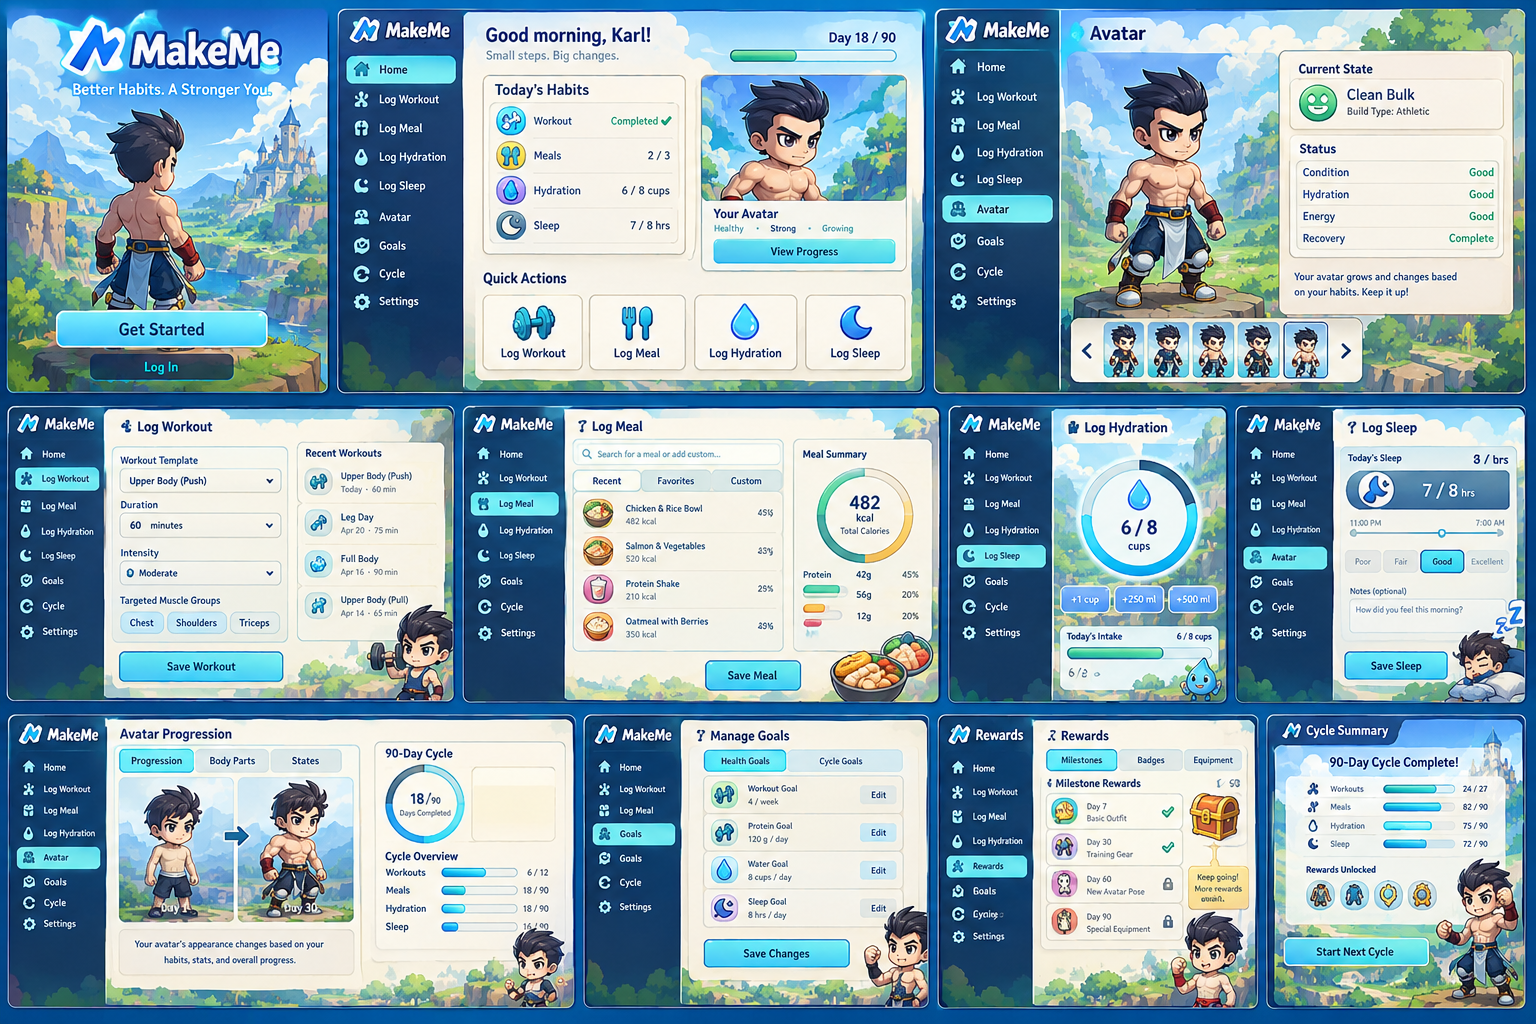
\includegraphics[width=0.82\linewidth]{figures/feasibility-evidence.png}
    }{
        \figureplaceholder{45mm}{Add supporting feasibility evidence here.}
    }
    \caption{Supporting feasibility evidence for the proposed project.}
    \label{fig:feasibility}
\end{figure}

% Example for a borrowed/adapted image:
% \caption{Existing system architecture, adapted from \cite{demoDocs2026}.}

% ============================================================
% 6. Resources and Risks
% ============================================================
\section{Resources and Risks}

% Identify required software, data, hardware, APIs, accounts, licenses,
% or other resources.
%
% Identify at least two meaningful risks or constraints and explain
% how each could be reduced or handled.

\begin{table}[H]
    \centering
    \caption{Initial project risks and mitigation strategies.}
    \label{tab:risks}
    \begin{tabularx}{\textwidth}{
        >{\raggedright\arraybackslash}p{0.27\textwidth}
        >{\raggedright\arraybackslash}p{0.29\textwidth}
        >{\raggedright\arraybackslash}X
    }
        \toprule
        \textbf{Risk / Constraint} &
        \textbf{Why it matters} &
        \textbf{Mitigation / Fallback} \\
        \midrule
        Replace with risk 1 &
        Explain the impact &
        Explain how the risk could be reduced or handled. \\
        \addlinespace
        Replace with risk 2 &
        Explain the impact &
        Explain how the risk could be reduced or handled. \\
        \bottomrule
    \end{tabularx}
\end{table}

% ============================================================
% References
% ============================================================
\printbibliography[title={References}]

\end{document}
